\documentclass{beamer}
\usetheme{Antibes}
\usepackage{subcaption}
\usepackage{amsmath, amsfonts, amssymb}
\usepackage{physics}
\setbeamertemplate{footline}[frame number]
\setbeamersize{text margin left=5mm} 

\AtBeginSection[]{
  \begin{frame}
  \vfill
  \centering
  \begin{beamercolorbox}[sep=8pt,center,shadow=true,rounded=true]{title}
    \usebeamerfont{title}\insertsectionhead\par%
  \end{beamercolorbox}
  \vfill
  \end{frame}
}

\DeclareMathOperator*{\argmin}{arg\,min}

\title{Classification of modern ML algorithms}
\subtitle{Following \textit{Beyond Euclid:
An Illustrated Guide to Modern Machine Learning
with Geometric, Topological, and Algebraic Structures} by Sanborn et al.}
\author{Presented by: Evgenii Samutichev}

\begin{document}

\maketitle

\begin{frame}{Outline}
    \small 
    \tableofcontents
\end{frame}

\section{Classification as Mathematician's endeavor }
\begin{frame}{Classification as Mathematician's endeavor}{Square matrices}
  \begin{itemize}
    \item \textbf{Square matrices} are everywhere in applied mathematics
    \item Different matrices, but the same \textbf{operator}
    \item Some aspects might not be captured exactly, e.g. $\kappa_2(J) \neq \kappa_2(A)$
  \end{itemize}
  \begin{figure}[h!]
    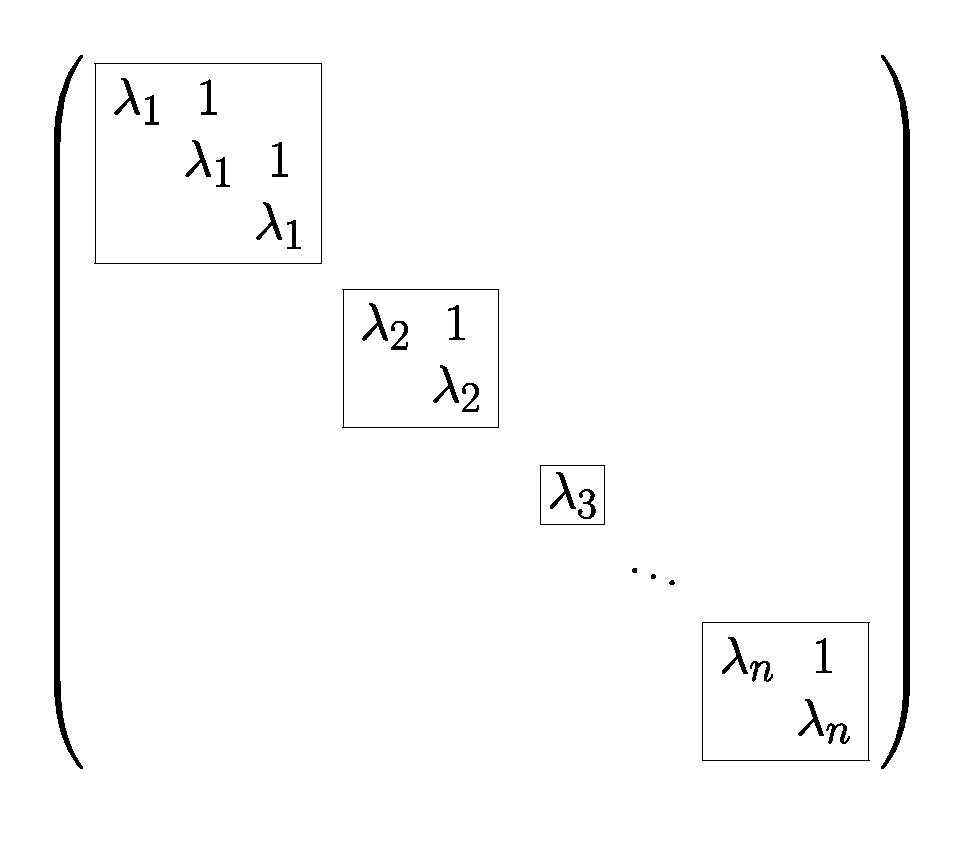
\includegraphics[width=0.4\textwidth]{images/Jordan_canonical_form.pdf}
    \caption{\textbf{Jordan normal form} (1870) by Camille Jordan. There is nothing, but blocks in this realm.}
  \end{figure}
\end{frame}

\begin{frame}{Classification as a Mathematician's endeavor}{Hilbert spaces}
  \begin{itemize}
    \item \textbf{Separable Hilbert spaces}\footnote{In QM they include finite-dimensional inner product spaces to this notion} over $\mathbb{C}$ are widely used in Quantum Mechanics to represent \textbf{state spaces} 
    \item Separable $\iff$ at most countable orthonormal basis 
    \item Up to an isomorphism that's all there is:
  \end{itemize}
  \begin{align*}
    \mathbb{C}, \mathbb{C}^2, ..., \mathbb{C}^n, ... \quad  \underbrace{\ell^2(\mathbb{C})}_{\text{the one and only } \infty\text{-dimensional} }
  \end{align*}
\end{frame}

\begin{frame}{Classification as a Mathematician's endeavor}{Groups}
  \begin{itemize}
    \item \textbf{Groups} as algebraic objects used to express \textbf{symmetries}
  \end{itemize}
  \begin{figure}[h!]
    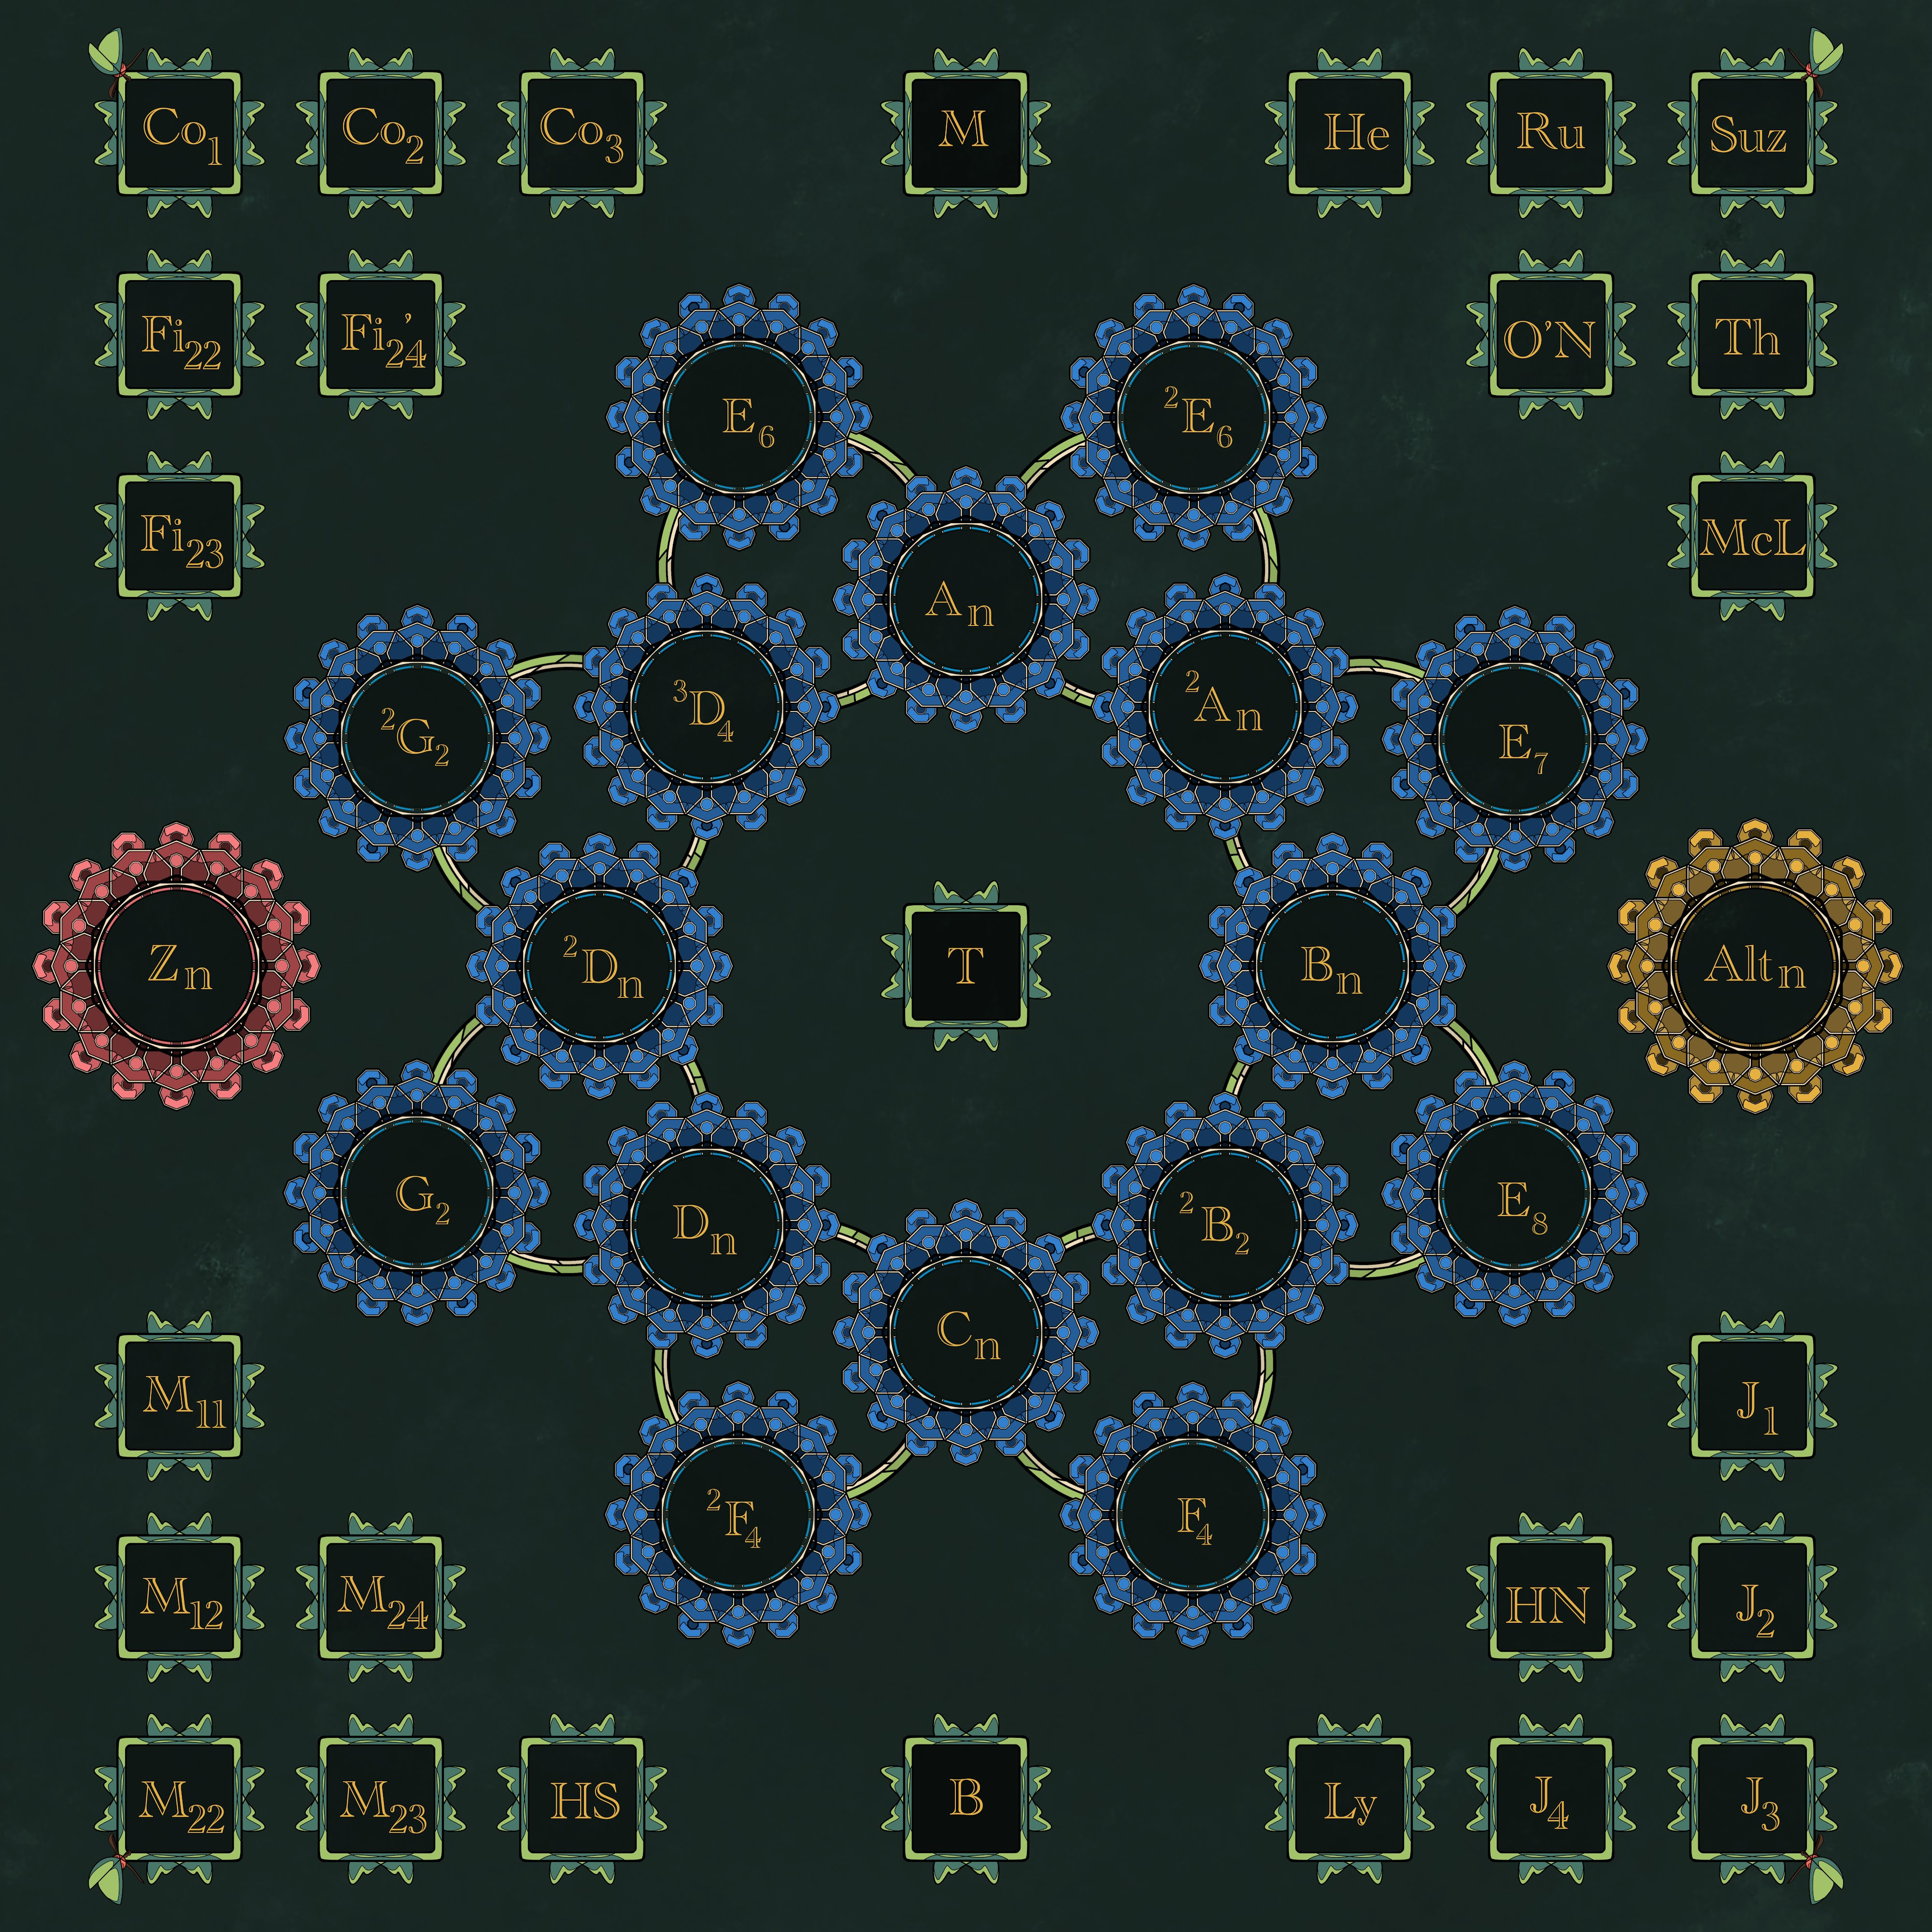
\includegraphics[width=0.4\textwidth]{images/Classification_of_the_finite_simple_groups.png}
    \caption{\textbf{Classification of finite simple groups} (2004). Thousands of pages, about a hundred authors -- all to yield this power...}
  \end{figure}
\end{frame}

\section{Textbook classification of ML algorithms}

\begin{frame}{Textbook classification of ML algorithms}
  
\begin{itemize}
  \item Two dimensions: 
  \begin{enumerate}
    \item set of \textbf{labels} $y_i$: complete, some, $\varnothing$
    \item type of labels: typically either $\mathcal{Y}=\{1,2,3,...,k\}$ or $\mathcal{Y}=\mathbb{R}^n$
  \end{enumerate} 
  \item Glaring issue: not mentions the \textbf{structure} of $\mathcal{X}$
  \item What is \textbf{reinforcement learning} even doing here?
\end{itemize}
\begin{figure}
  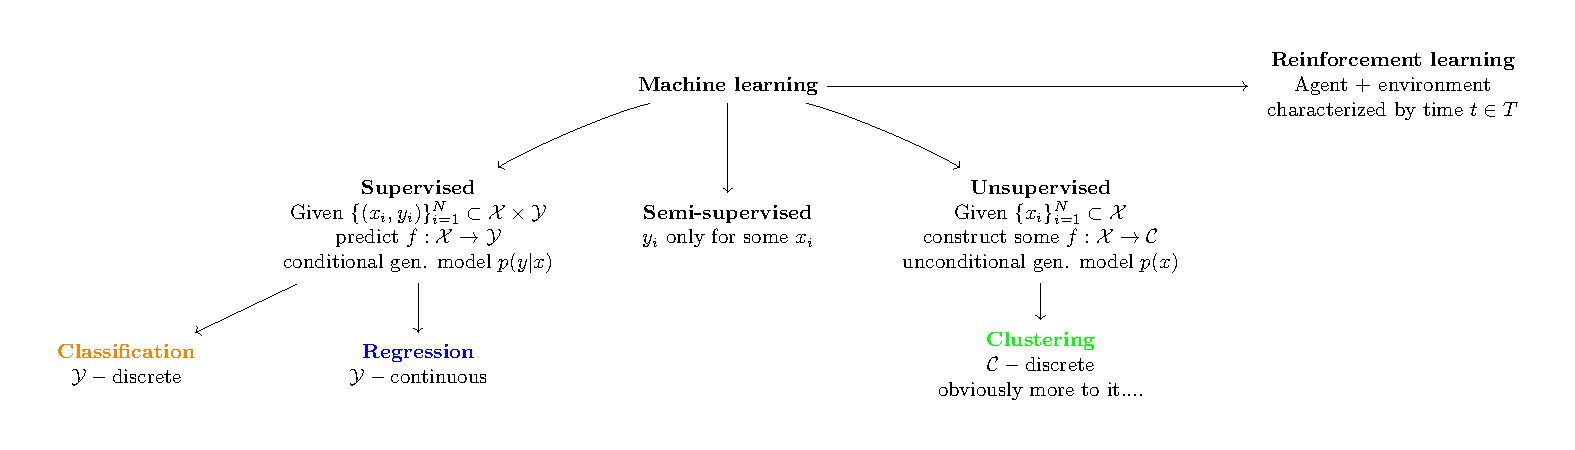
\includegraphics[width=1.1\textwidth]{images/ML_classification_1.pdf}
  \caption{Good ol' classification}
\end{figure}
\end{frame}

\section{Classification of data}
\subsection{Structure in data}
\subsubsection{Topology}
\begin{frame}{Structure in data}{Topology: Relationships (1 / 2)}
\begin{itemize}
  \item A \textbf{topological space} is a pair $(\Omega, \tau)$, where $\Omega$ is a set, while $\tau \subset 2^\Omega$ is known as \textbf{topology} that contains so called \textit{open sets}, essentially \textbf{neighborhoods} of points in $\Omega$. 
  \item Formally, $\tau$ must contain at least $\varnothing$ and $\Omega$, and be closed w.r.t. any unions and finite intersections.
  \item Examples: 
  \begin{enumerate}
    \item All metric spaces $(X, d)$, particularly \textbf{graphs} where $d(v, w)$ is the length of a shortest path between two nodes $v$ and $w$
    \item \textbf{Hypergraphs}: non-metrizable, e.g. Sierpiński space $\Omega = \{\circ,\bullet\}, \tau = \{\varnothing, \{\circ\}, \{\circ,\bullet\} \}$
  \end{enumerate}
\end{itemize}
\begin{figure}
  \centering
  \begin{subfigure}{.5\textwidth}
    \centering
    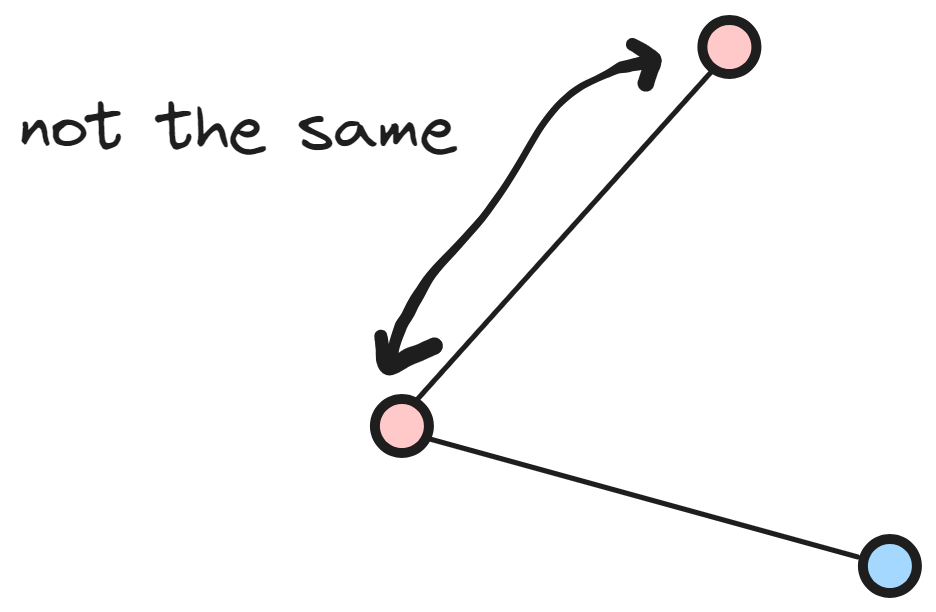
\includegraphics[width=.4\linewidth]{images/graph1.png}
    \caption{Graph structure in data}
  \end{subfigure}%
  \begin{subfigure}{.5\textwidth}
    \centering
    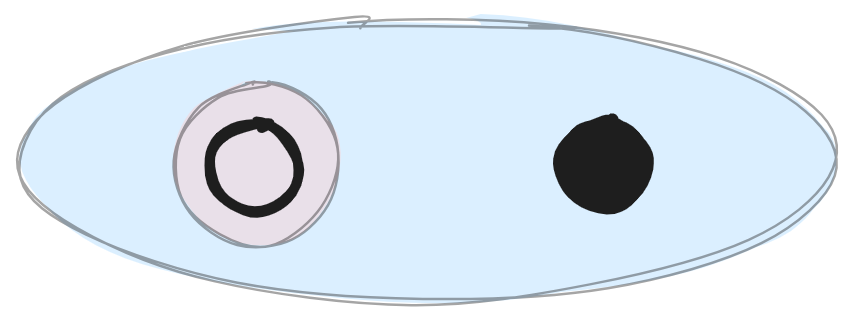
\includegraphics[width=.4\linewidth]{images/Sierpinski.png}
    \caption{Sierpiński space, open sets as hyperedges}
  \end{subfigure}
  \caption{Graphs and hypergraphs}
  \end{figure}
\end{frame}

\begin{frame}{Structure in data}{Topology: Relationships (1 / 2)}
\begin{itemize}
  \item A \textbf{topological space} is a pair $(\Omega, \tau)$, where $\Omega$ is a set, while $\tau \subset 2^\Omega$ is known as \textbf{topology} that contains so called \textit{open sets}, essentially \textbf{neighborhoods} of points in $\Omega$. 
  \item Formally, $\tau$ must contain at least $\varnothing$ and $\Omega$, and be closed w.r.t. any unions and finite intersections.
  \item Examples: 
  \begin{enumerate}
    \item All metric spaces $(X, d)$, particularly \textbf{graphs} where $d(v, w)$ is the length of a shortest path between two nodes $v$ and $w$
    \item \textbf{Hypergraphs}: non-metrizable, e.g. Sierpiński space $\Omega = \{\circ,\bullet\}, \tau = \{\varnothing, \{\circ\}, \{\circ,\bullet\} \}$
  \end{enumerate}
\end{itemize}
\begin{figure}
  \centering
  \begin{subfigure}{.5\textwidth}
    \centering
    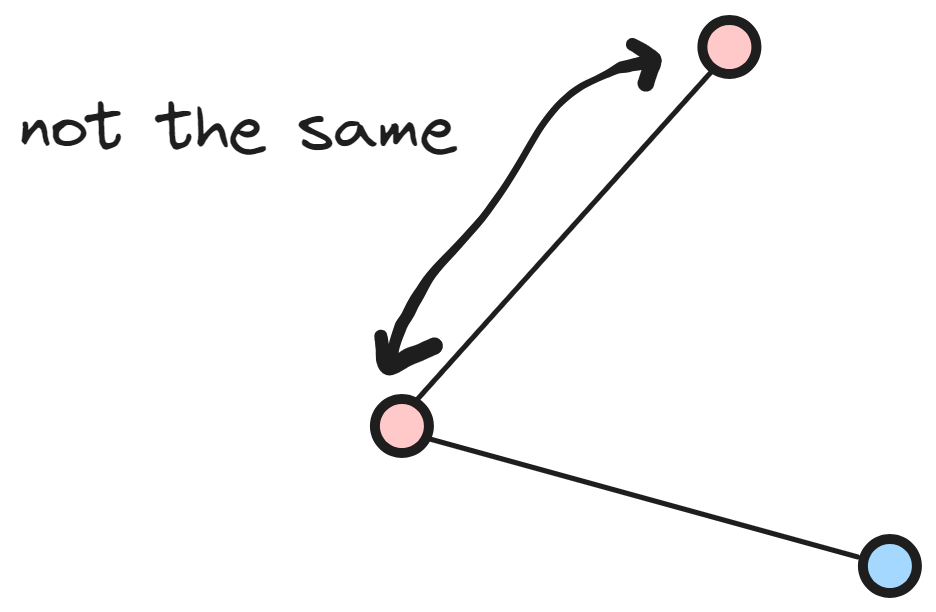
\includegraphics[width=.4\linewidth]{images/graph1.png}
    \caption{Graph structure in data}
  \end{subfigure}%
  \begin{subfigure}{.5\textwidth}
    \centering
    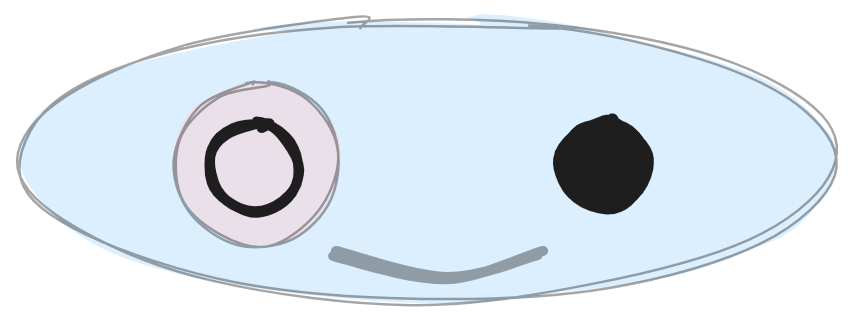
\includegraphics[width=.4\linewidth]{images/Sierpinski_meme.png}
    \caption{Sierpiński space, open sets as hyperedges}
  \end{subfigure}
  \caption{Graphs and hypergraphs}
  \end{figure}
\end{frame}
  
\begin{frame}{Structure in data}{Topology: Relationships (2 / 2)}
\begin{itemize}
  \item Topology emphasizes \textbf{relationships} in data
  \item We will only consider \textbf{discrete} topological structures, something like $(\mathbb{R}, |\cdot|)$ is not particularly interesting in the context of relationships as it's too homogenous
\end{itemize}
  \begin{figure}[h!]
    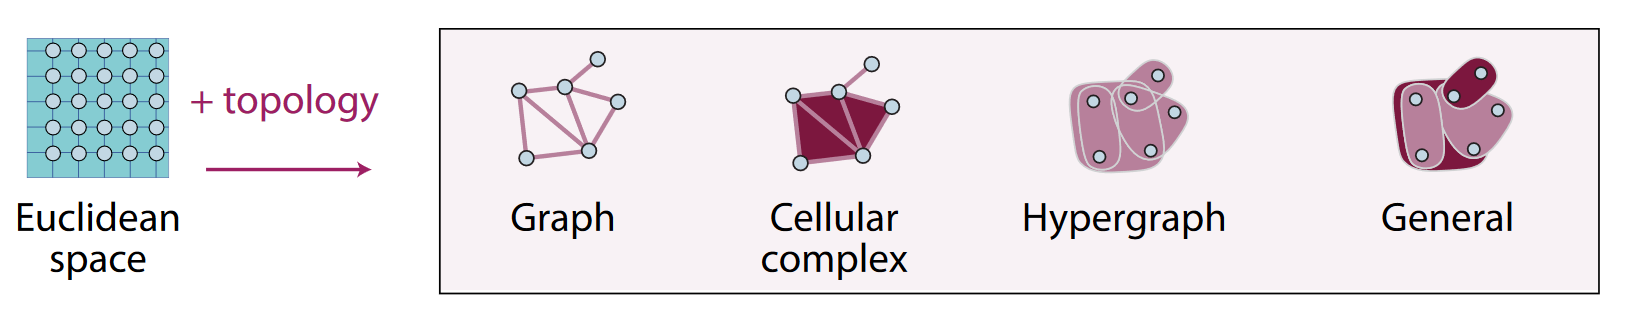
\includegraphics[width=0.8\textwidth]{images/es_topology.png}
    \caption{From the paper,/ kinds of \textbf{topological} structures one can impose}
  \end{figure}
\end{frame}

\subsubsection{Geometry}
\begin{frame}{Structure in data}{Geometry: Measurements (1 / 2)}
\begin{itemize}
  \item A \textbf{manifold} is a continuous\footnote{as opposed to discrete that we just discussed} topological space $(M, \tau)$, that locally resembles Euclidean space $\left(\mathbb{R}^n, \langle \cdot, \cdot \rangle\right)$.
  \item Formally: for every $x \in M$ there exists $U \in \tau$ s.t. $x \in U$ and there exists $f: U \to V \subset \mathbb{R}^n$ continuous, invertible, $f^{-1}$ is continuous (homeomorphism).
  \item Why do we care about \textbf{geometry}? For one thing -- it helps to compress data
\end{itemize}
\begin{figure}[h!]
  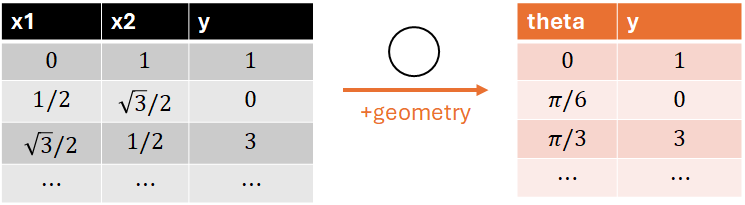
\includegraphics[width=0.6\textwidth]{images/geometry_data.png}
  \caption{$x_1, x_2$ are nothing more than $\sin\theta, \cos \theta$, so we only need 1 parameter}
\end{figure}
\end{frame}

\begin{frame}{Structure in data}{Geometry: Measurements (2 / 2)}
\begin{itemize}
  \item We will focus on a subclass of \textbf{Riemannian manifolds} $(M, g)$, which are smooth manifolds equipped with an inner product $g : M \to \langle \cdot, \cdot\rangle_{p}$ on the tangent space at every point called \textbf{Riemannian metric}
  \item Geometry reveals the nature of \textbf{measurements} in the dataset, e.g. \textbf{geodetic data}
\end{itemize}
\begin{figure}[h!]
  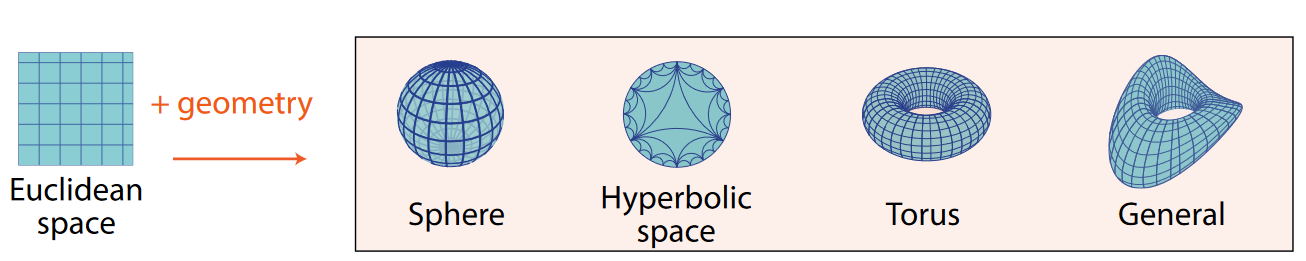
\includegraphics[width=0.8\textwidth]{images/es_geometry.png}
  \caption{From the paper, kinds of \textbf{geometric} structures one can impose}
\end{figure}
\end{frame}

\subsubsection{Algebra}
\begin{frame}{Structure in data}{Algebra: Transformations (1 / 2)}
  \begin{itemize}
    \item A \textbf{group} is a set of invertible transformations that can be composed.
    \item Formally: a group is a pair $(G, *)$ of a set together with an associative operation $* : G \times G \to G$ s.t. there exists $e \in G$ s.t. $g * e = e * g = g$, and for all $g \in G$ there exists $g^{-1}$ s.t. $g * g^{-1} = g^{-1} * g = e$.
    \item Example: a triangle group
  \end{itemize}
  \begin{figure}[h!]
    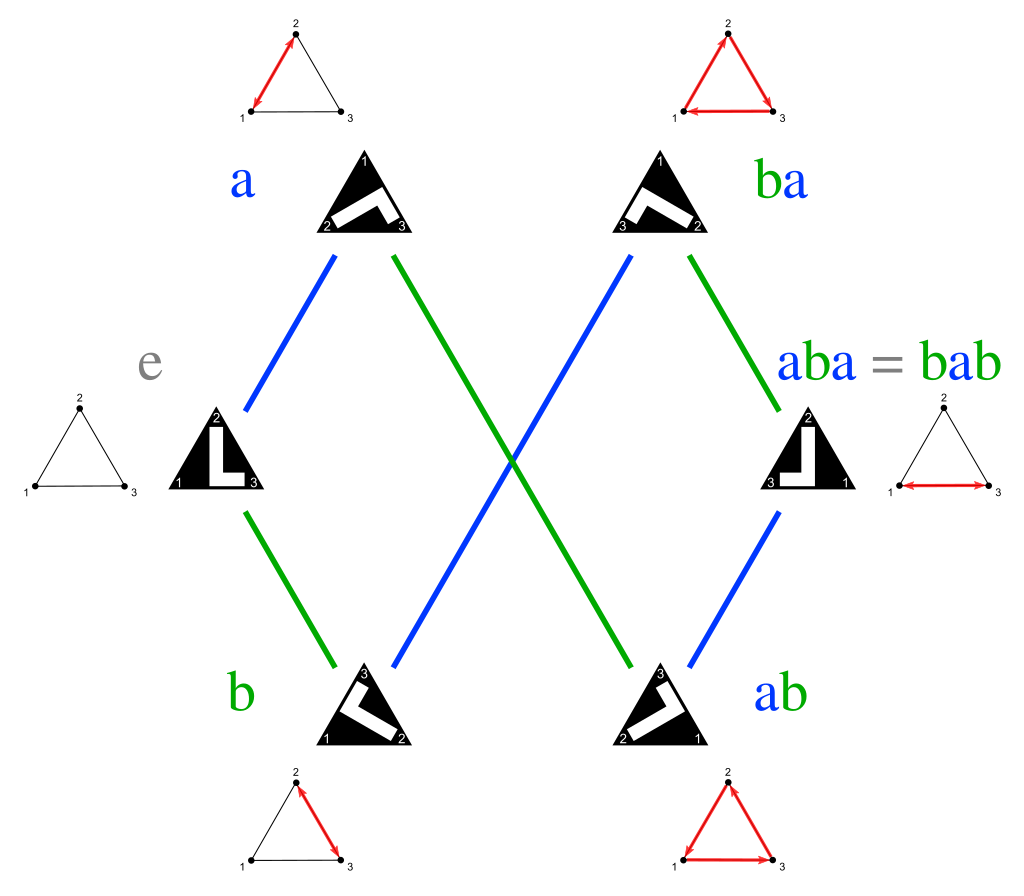
\includegraphics[width=0.28\textwidth]{images/Cayley_graph_of_S3_with_triangles.png}
    \caption{Algebraic description of an equilateral triangle's symmetries}
  \end{figure}
\end{frame}

\begin{frame}{Structure in data}{Algebra: Transformations (2 / 2)}
  \begin{itemize}
    \item \textbf{Lie groups} are groups representing continuous transformations.
    \item Example: translations and rotations of Euclidean plane
    \item A group $G$ exists a separate entity from an object $X$ that it can transform, but if we want to emphasize this aspect, than we use a so called \textbf{group action} $G \times X \to X$. 
    \item Groups allow us to talk about transformation \textbf{invariances,} \textbf{equivariances}, etc. 
  \end{itemize}
  \begin{figure}[h!]
    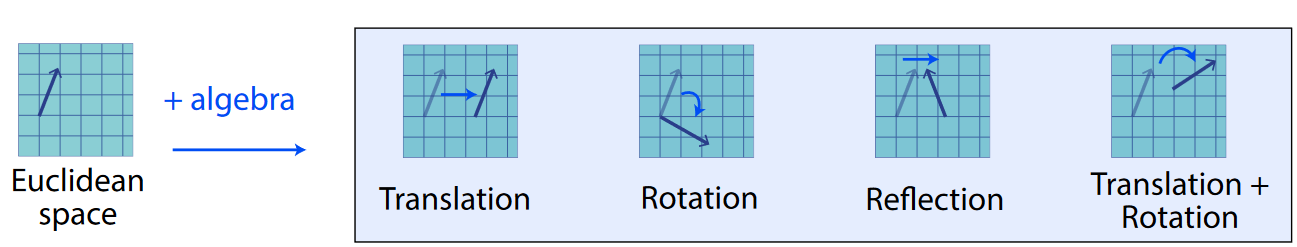
\includegraphics[width=0.8\textwidth]{images/es_algebra.png}
    \caption{From the paper, kinds of \textbf{algebraic} structures one can impose}
  \end{figure}
\end{frame}
  
\subsection{Data as coordinates in space}
\begin{frame}{Data as coordinates in space}{Examples (1 / 2)}
\begin{itemize}
  \item A given data entry $x_i$ represents \textbf{coordinates} of a point in some space $X$
  \item Implicitly assumes the existence of a \textbf{coordinate system}, typically in the form of \textbf{units of measurement}
\end{itemize}
\begin{figure}[h!]
  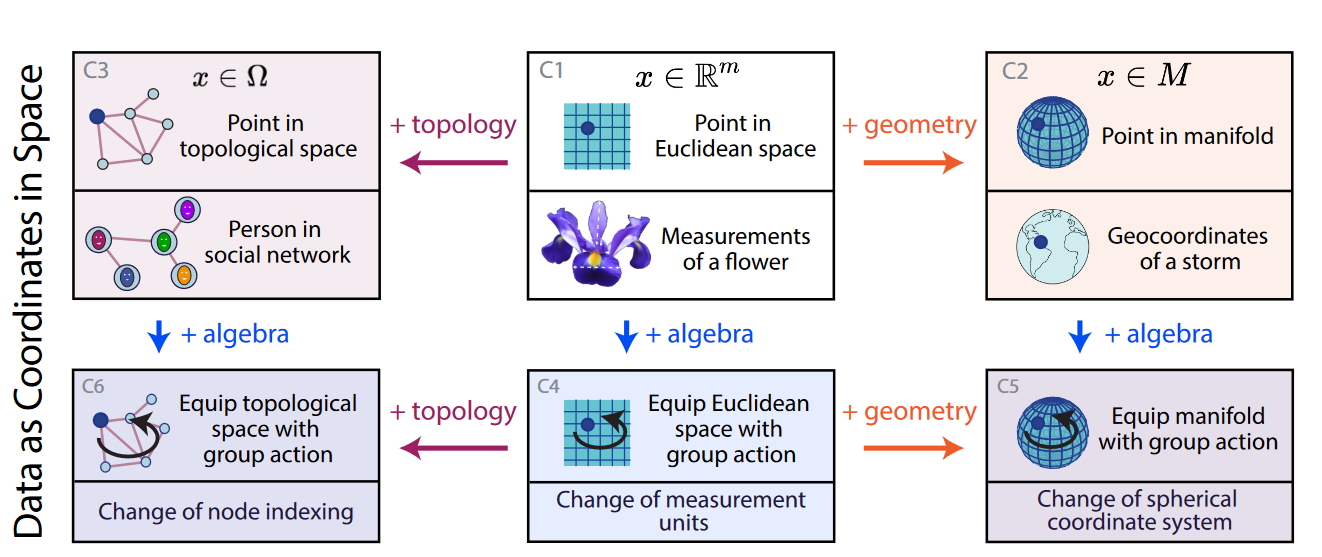
\includegraphics[width=0.8\textwidth]{images/data_coordinates.png}
  \caption{From the paper, structures in data and their compositions}
\end{figure}
\end{frame}

\begin{frame}{Data as coordinates in space}{Examples (2 / 2)}
\begin{itemize}
  \item A simple example where recognizing a topological structure is beneficial.
  \item One can use \textbf{centrality measures} to identify key members of an organization, that connect other people.
  \item One might also count the number of layers, and so on.
\end{itemize}
\begin{figure}[h!]
  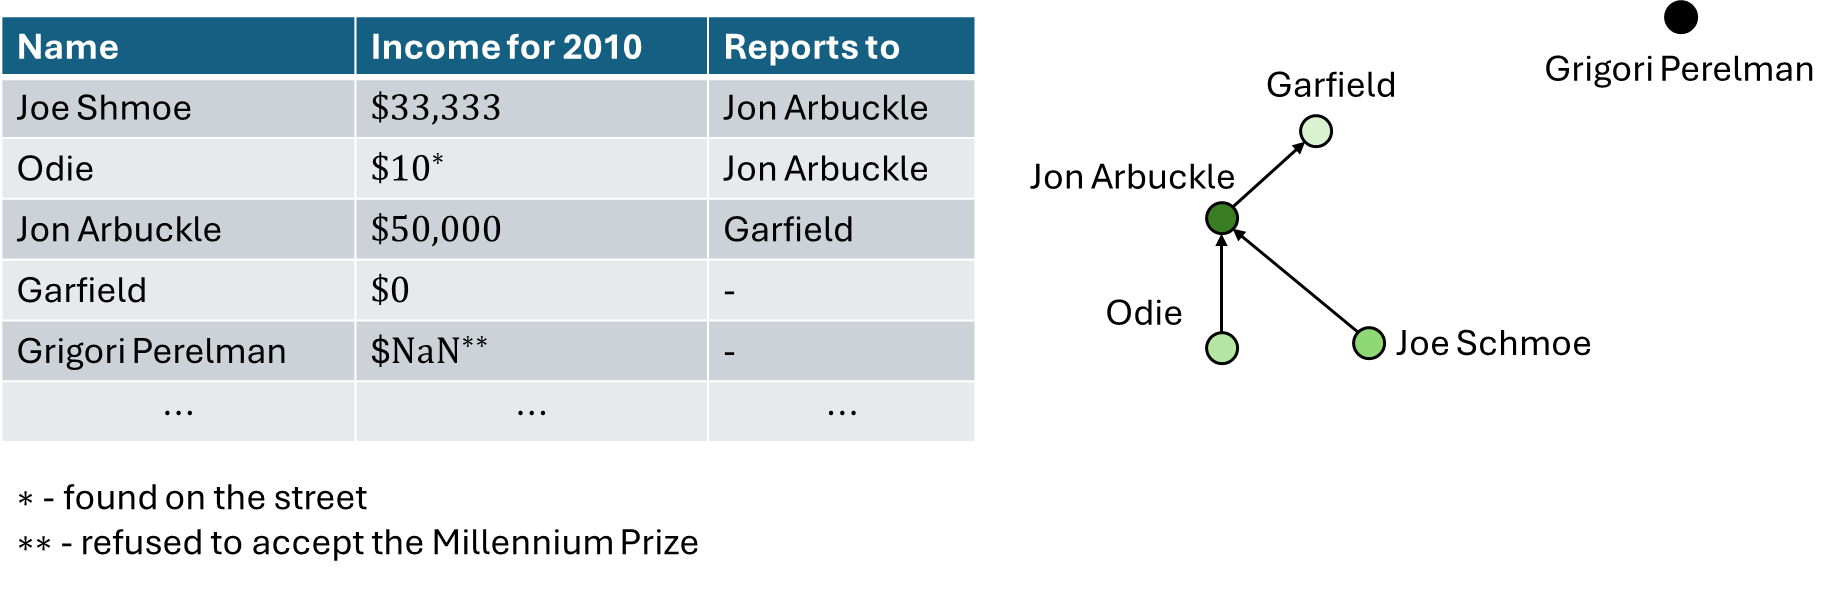
\includegraphics[width=0.8\textwidth]{images/topology_data.png}
  \centering 
  \caption{Some fictional cooperative, any similarity to names or incedents is entirely coincidental}
\end{figure}
\end{frame}

\begin{frame}{Data as coordinates in space}{Non-Euclidean Probability and Statistics}
\begin{itemize}
  \item If data is equipped with some geometric structure $(M, g)$, we need to rethink what a \textbf{mean} means. 
  \item Let $d(x, y)$ be the geodesic distance between $x, y \in M$. Introducing \textbf{the Fréchet mean}
\end{itemize}
\begin{align}
 \mu
    &= \arg \min_{x \in M}{\sum_{i=1}^{n}{d(x_i, x)^2}},
\end{align}
\begin{minipage}{.5\textwidth}
  \begin{figure}[h!]
    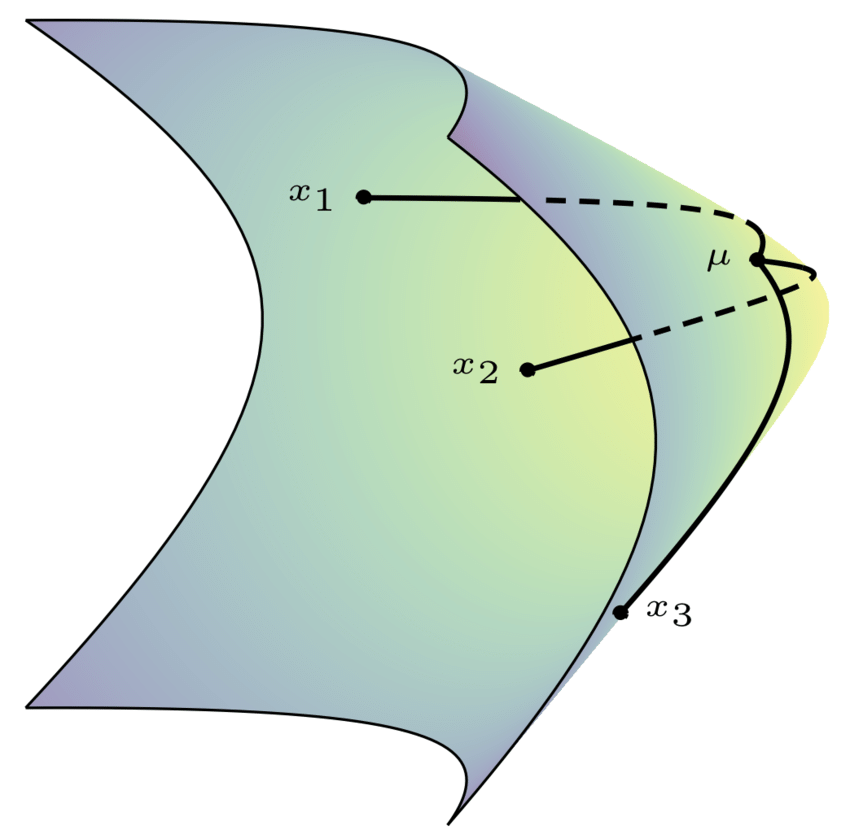
\includegraphics[width=0.6\textwidth]{images/frechet mean.png}
    \centering
  \end{figure}
\end{minipage}%
\begin{minipage}{.5\textwidth}
    \centering
    \begin{figure}[h!]
      \raggedleft
      
\includegraphics[width=.7\linewidth]{images/meme.jpg}
    \end{figure}
\end{minipage}
\end{frame}

\subsection{Data as signals}
\begin{frame}{Data as signals (1 / 2)}
\begin{itemize}
  \item A given data entry $x_i$ represents a whole function $x_i : T \to X$ between two spaces, elements of $X$ are called \textbf{values} of the \textbf{signal} $x$.
  \item $T$ might represent time, or it might be a position on an image.
  \item $X$ might represent wave amplitude and phase, or it might be a triplet of colors.
  \item Example: a grayscale image $x : \mathbb{R}^2 \to \mathbb{R}$  
\end{itemize}
\begin{minipage}{.5\textwidth}
  \begin{figure}[h!]
    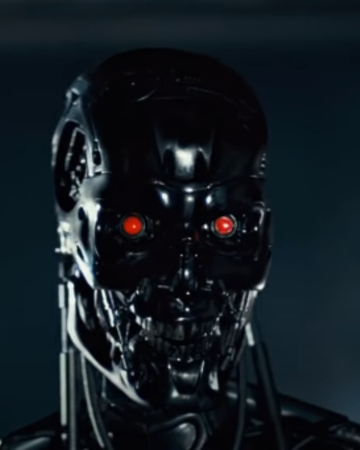
\includegraphics[width=0.4\textwidth]{images/image.png}
    \centering
  \end{figure}
\end{minipage}%
\begin{minipage}{.5\textwidth}
    \centering
    \begin{figure}[h!]
      \raggedleft
      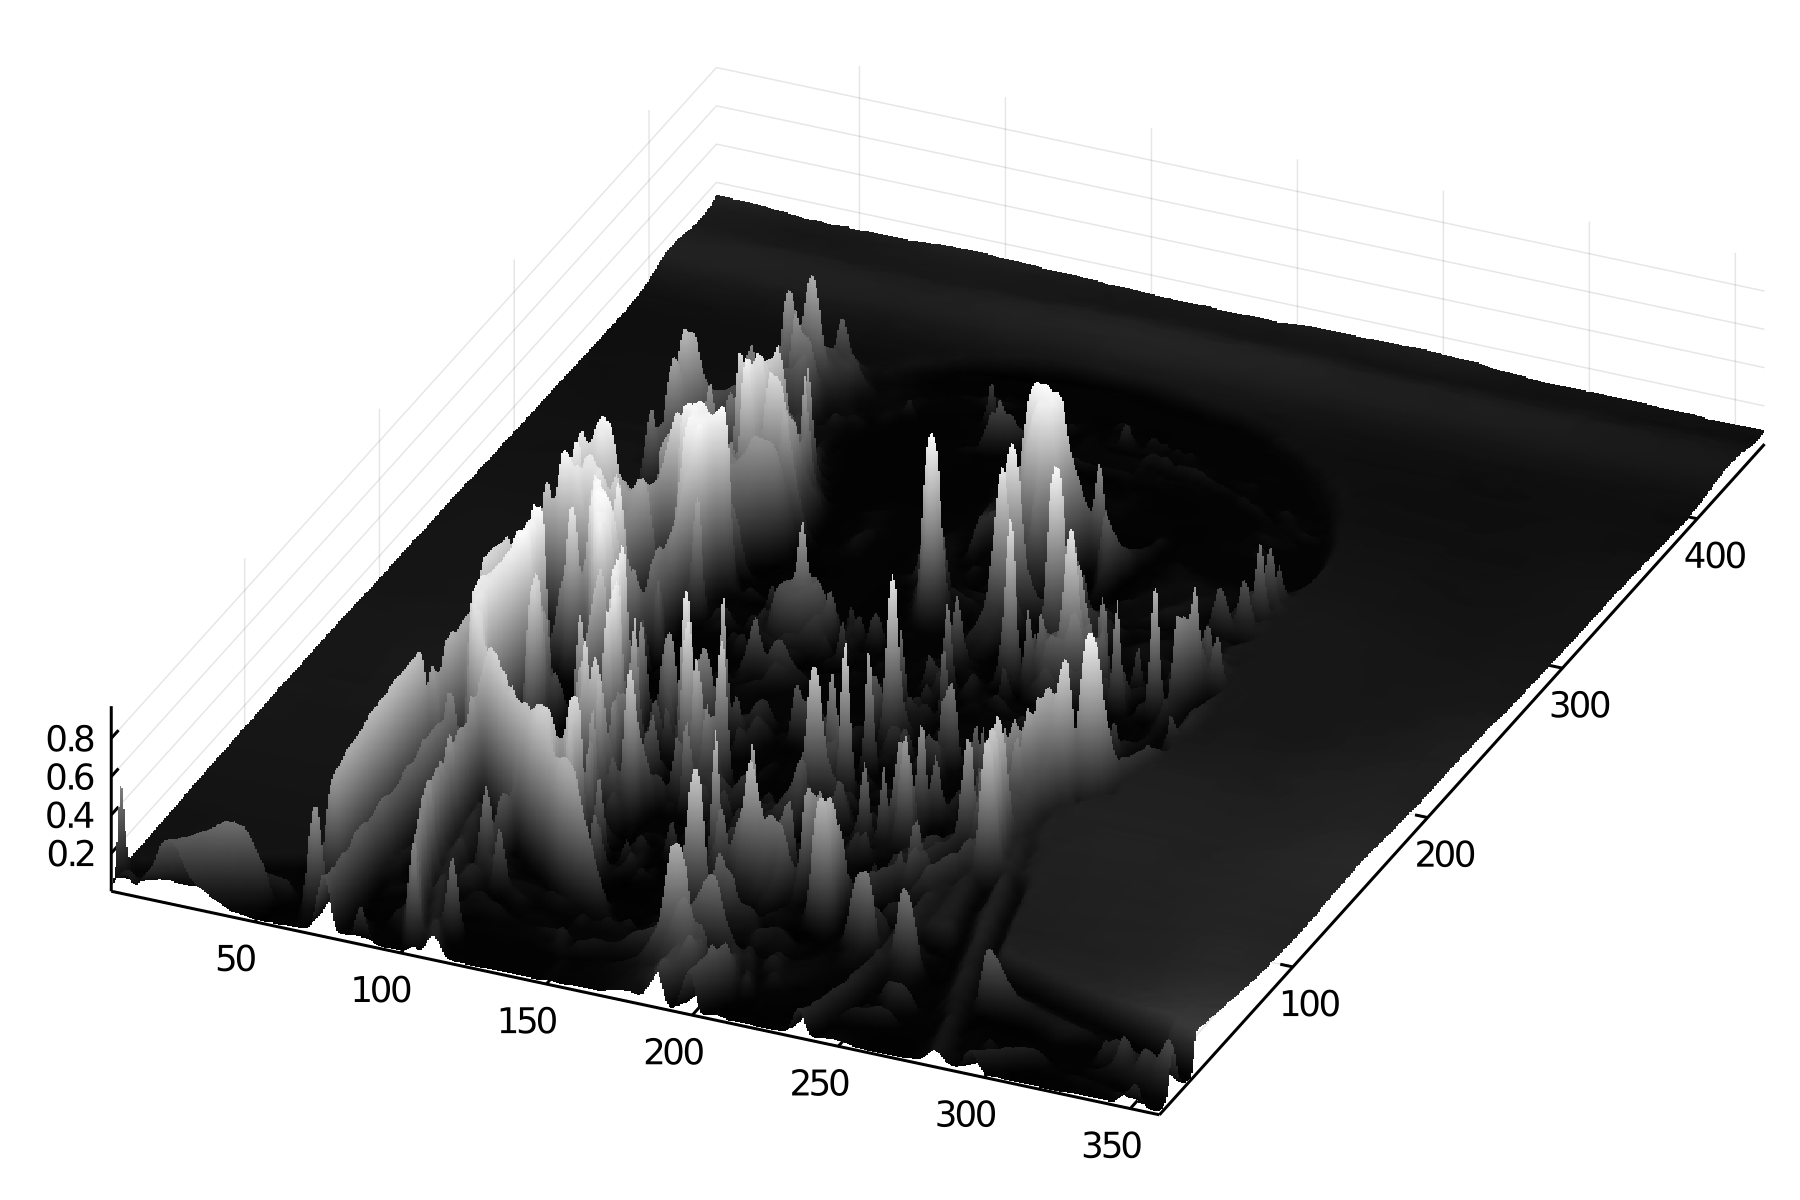
\includegraphics[width=.7\linewidth]{images/result1.png}
    \end{figure}
\end{minipage}
\end{frame}

\begin{frame}{Data as signals (2 / 2)}
\begin{figure}[h!]
  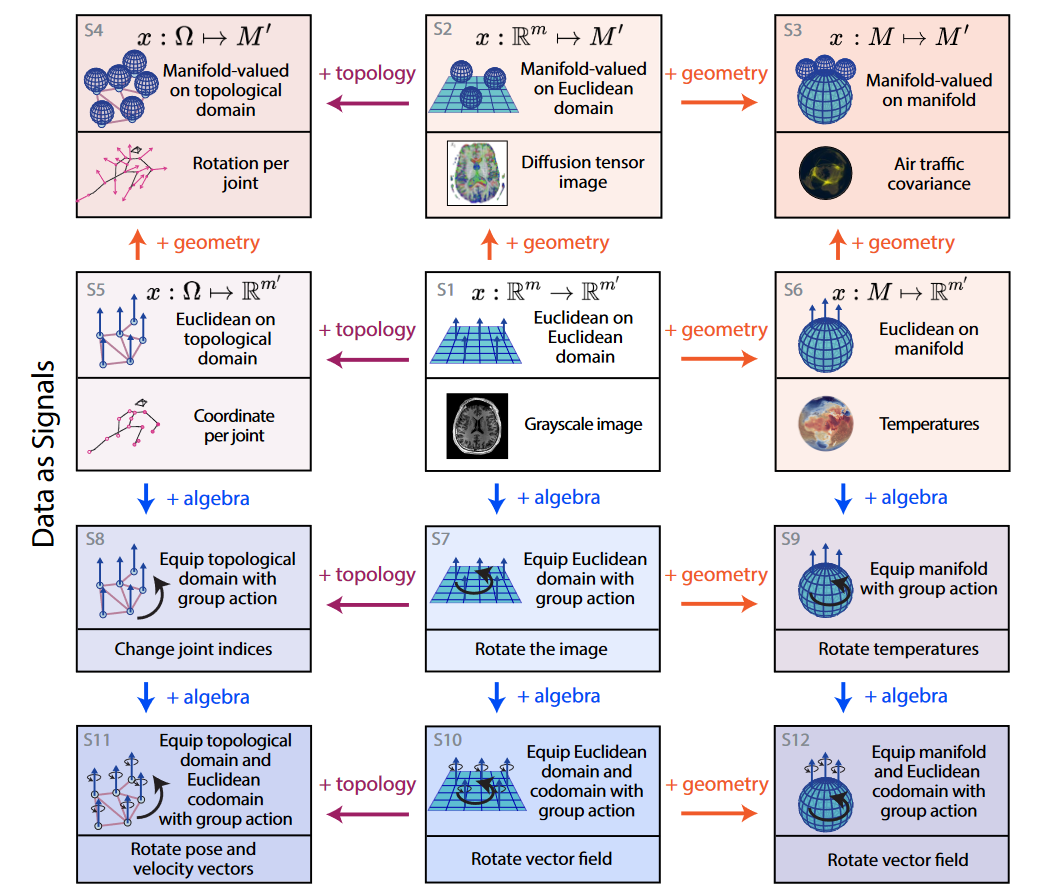
\includegraphics[width=0.7\textwidth]{images/data_signals.png}
  \caption{From the paper, structures in data and their compositions}
\end{figure}
\end{frame}

\subsubsection{Notable examples}

\begin{frame}{Data as signals}{Notable examples}
  \begin{minipage}{.5\textwidth}
    \begin{figure}[h!]
      \centering 
      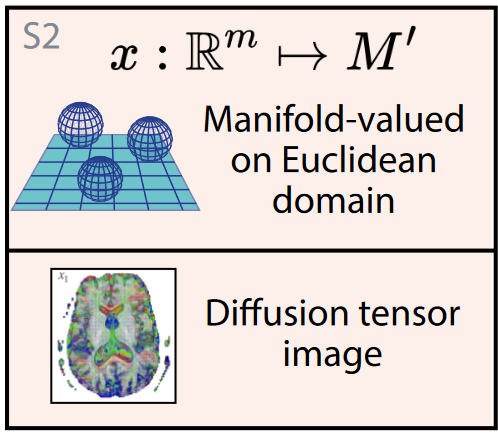
\includegraphics[width=.7\linewidth]{images/manifold_on_euclidean.png}
      \caption{$M'=\text{SPD}(3)$  -- covariance matrices describe how molecules diffuse in the brain}
    \end{figure}
  \end{minipage}%
  \begin{minipage}{.5\textwidth}
      \begin{figure}[h!]
        \centering
        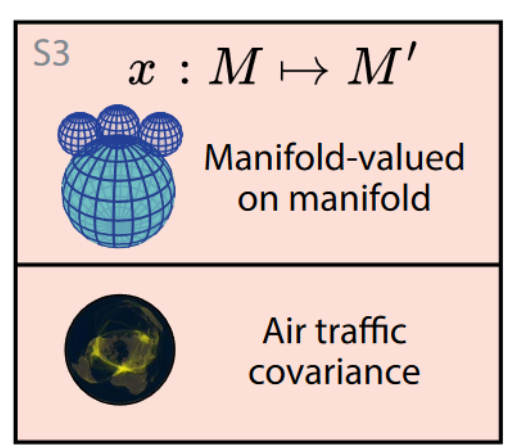
\includegraphics[width=0.6\textwidth]{images/manifold_to_manifold.png}
        \centering
        \caption{$M = S^2$ -- Earth surface, $M'=\text{SPD}(2)$ -- covariances of speed vectors of the aircraft}
    \end{figure}
\end{minipage}
\end{frame}

\begin{frame}{What to do when the structure is unknown}
\begin{itemize}
  \item For \textbf{topology}: \textbf{topological data analysis} allows to identify loops and other topological characteristics in data. 
  \item For \textbf{geometry}: \textbf{metric learning} allows to automatically construct task-specific distance metrics from data.
  \item For \textbf{algebra}: ?
\end{itemize}
\begin{figure}[h!]
  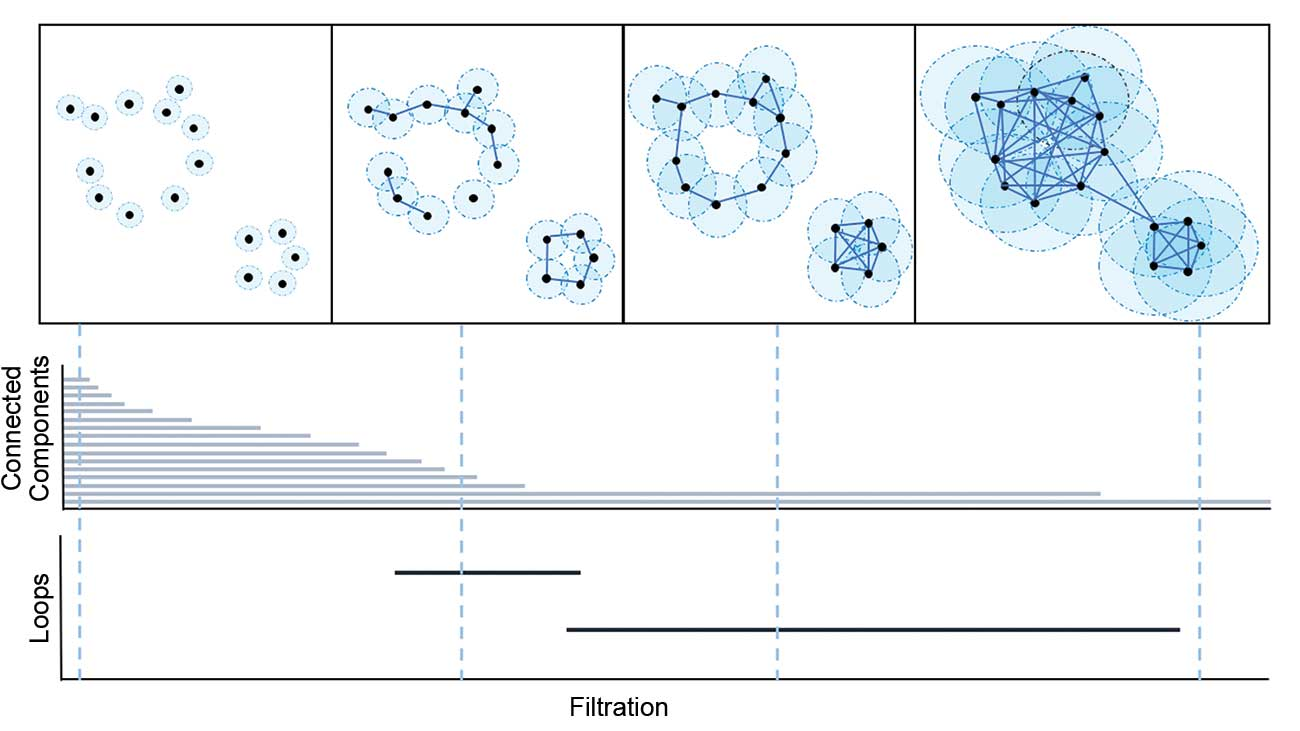
\includegraphics[width=0.5\textwidth]{images/barcode.jpg}
  \caption{Barcodes in TDA}
\end{figure}
\end{frame}

\section{Approaches to generalizing Euclidean models}
\begin{frame}{Approaches to generalizing Euclidean models}
\begin{itemize}
  \item \textbf{"Plug-In" methods}: replacing Euclidean notions of distance, mean, etc. with non-Euclidean counterparts. Examples:
  \begin{enumerate}
    \item k-nearest-neighbors on a manifold works with geodesic distance
    \item k-means on a manifold works with Fréchet mean 
  \end{enumerate}
  \item \textbf{Tangent space methods}: using the \textbf{exponential map} $\exp$ of the manifold (or rather its inverse), project on a tangent space and use Euclidean algorithms locally there. Examples:
  \begin{enumerate}
    \item Geodesic Regression
  \end{enumerate}
\end{itemize}
\end{frame}

\begin{frame}{Exponential map on a manifold (1 / 2)}
\begin{itemize}
  \item Let $(M, g)$ be a \textbf{geodesically complete} Riemannian manifold. For all $x \in M$ and $v_x \in T_x M$ there exists a unique geodesic $\gamma(t; x, v_x)$ defined for $t \in U \supset [0, 1]$ s.t. 
  \begin{align}
    \gamma(0; x, v_x) = x, \quad \gamma'(0; x, v_x) = v_x
  \end{align}
  \item Then, the exponential map $\exp : T M \to M$, where $T M := \{(x, v_x) \ | \ x \in M, v_x \in T_x M\}$ is defined as 
  \begin{align}
    \exp_x(v_x) 
      &= \gamma(1; p, v_x).
  \end{align}
\end{itemize}
\begin{figure}[h!]
  \centering 
  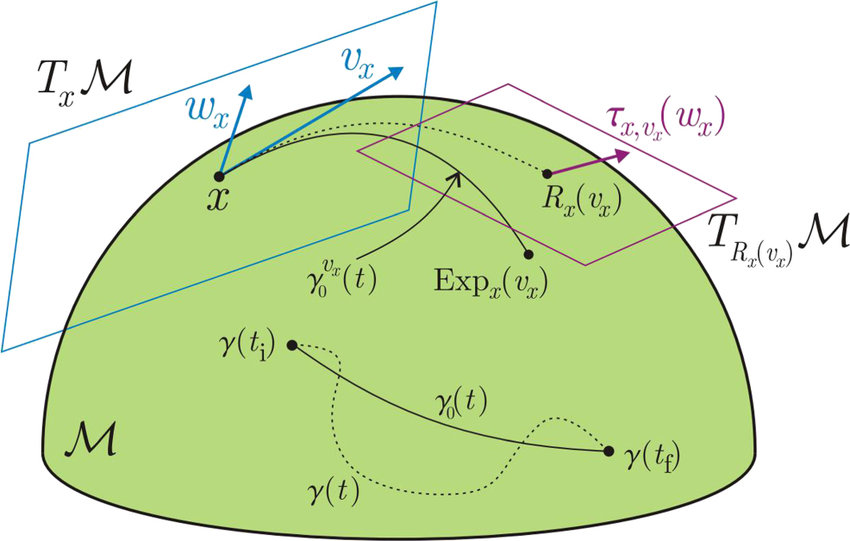
\includegraphics[width=0.4\textwidth]{images/expmap.png}
\end{figure}
\end{frame}

\begin{frame}{Exponential map on a manifold (2 / 2)}
  \begin{itemize}
    \item For $(\mathbb{R}^n, g_0)$, $g_0(x) = \langle \cdot, \cdot \rangle$ standard Euclidean metric,
    \begin{align}
      \exp_x(v_x) = x + v_x,
    \end{align}
    \item For $(S^1, d\theta \otimes d\theta)$ which we parametrize as $\text{e}^{i \theta}$, if $e=\text{e}^{0}$, then 
    \begin{align}
      \exp_e(v_x) = \text{e}^{i v_x},
    \end{align}
    \item In general, if $M=G$ as a matrix Lie group, then under a certain choice of Riemannian metric we have 
    \begin{align}
      \exp_e(A) = \text{e}^A,
    \end{align}
    matrix exponential, where $e\in G$ is the identity of the group. 
  \end{itemize}
\end{frame}

\begin{frame}{Geodesic regression }
  \begin{itemize}
    \item The \textbf{geodesic regression} was described for the first time in the work of Prof. Thomas Fletcher (2011)
    \item Let $X \in \mathbb{R}$ be an independent variable
    \item The regular regression is for a dependent variable $Y \in \mathbb{R}^n$, we are looking for $\alpha, \beta \in \mathbb{R}^n$ s.t. 
    \begin{align}
      Y = \alpha + X \beta + \epsilon,
    \end{align}
    \item The geodesic regression is for $Y \in M$ 
    \begin{align}
      Y = \exp(\exp(p, Xv), \epsilon),
    \end{align}
    for $(p, v) \in TM$ and $X \in \mathbb{R}$. Here $\exp(x, v_x) := \exp_x(v_x)$ in our previous notation. 
  \end{itemize}
\end{frame}

\section{Classification of regression algorithms}
\subsection{Euclidean to Euclidean}
\begin{frame}{Classification of regression algorithms}{Euclidean to Euclidean}
\begin{itemize}
  \item Bayesian methods integrate prior probabilistic distributions with observed data to update the model 
  \item Non-Bayesian, or frequentist, rely exclusively on observed data, without incorporating prior distributions on parameters 
\end{itemize}
\begin{figure}[h!]
  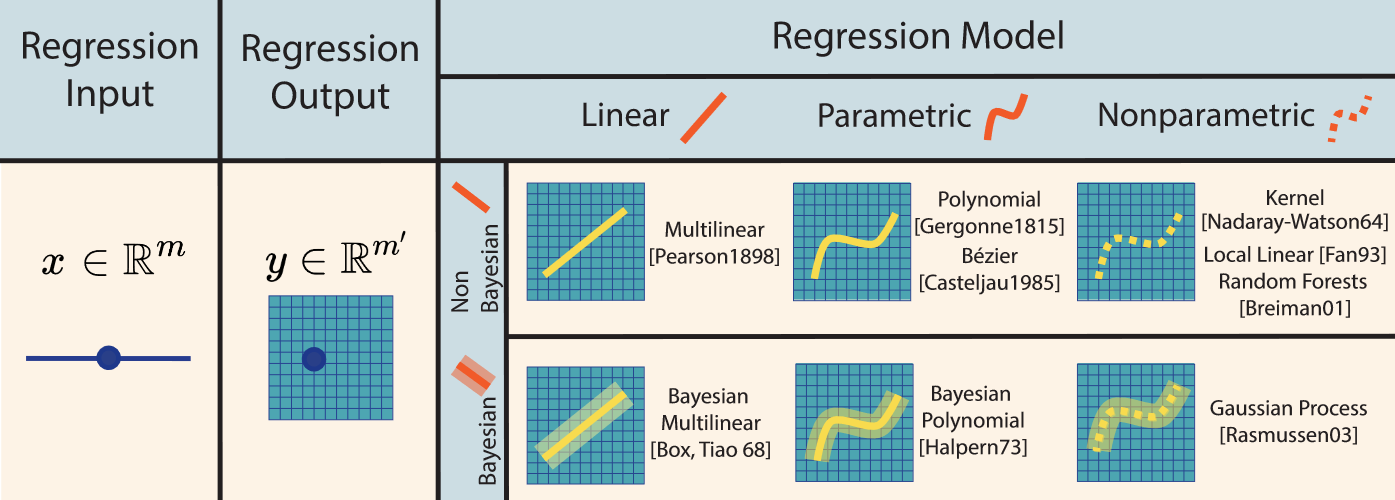
\includegraphics[width=0.8\textwidth]{images/regression_1.png}
\end{figure}  
\end{frame}

\subsection{Euclidean to non-Euclidean}
\begin{frame}{Classification of regression algorithms}{Euclidean to non-Euclidean}
\begin{itemize}
  \item \textbf{Fréchet regression} (by Petersen and Muller, 2016) generalizes the geodesic regression to higher-dimensional Euclidean inputs
  \item \textbf{Brownian motion} on a manifold for nonparametric (Wang and Lerman, 2015)
\end{itemize}
  \begin{figure}[h!]
    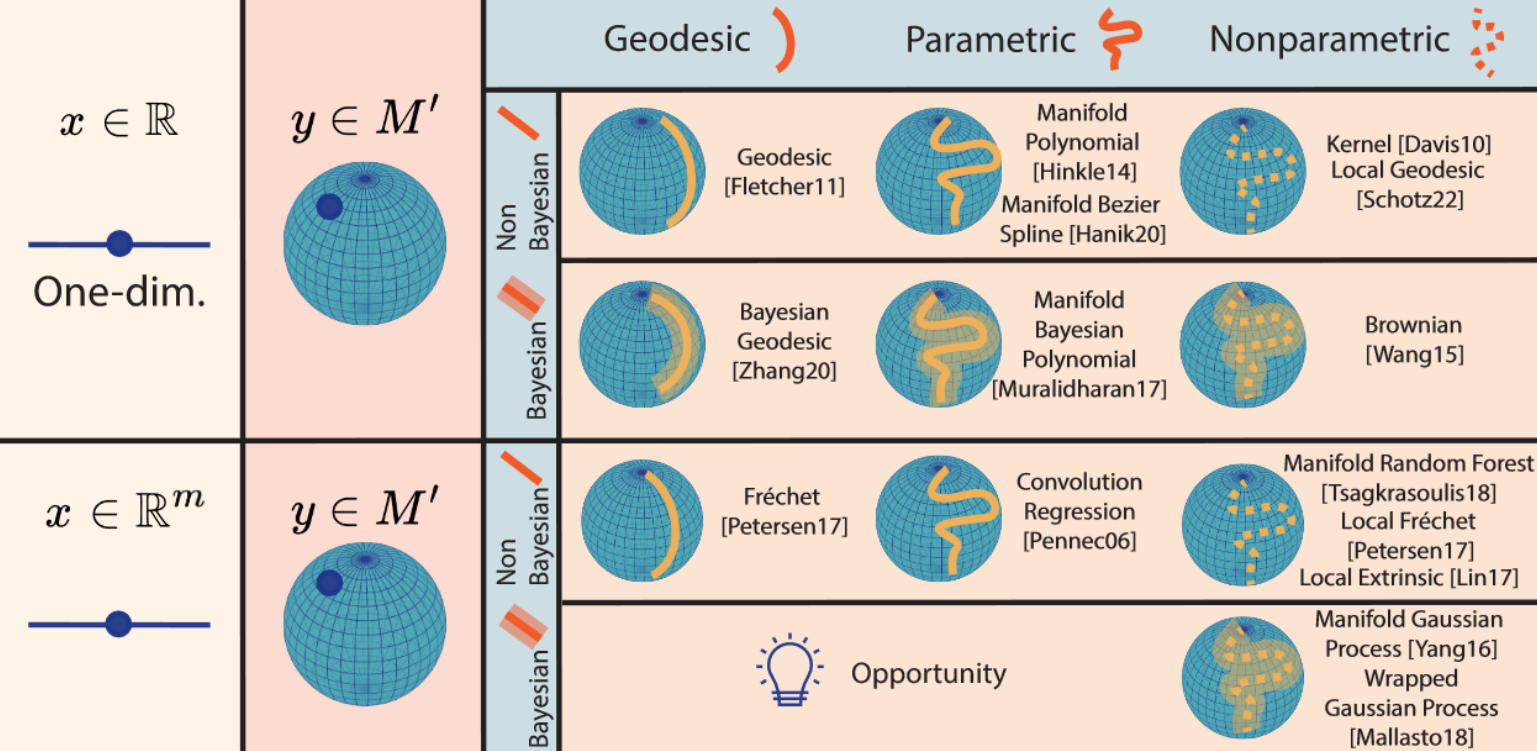
\includegraphics[width=0.8\textwidth]{images/regression_2.png}
  \end{figure}  
\end{frame}

\subsection{Non-Euclidean to Euclidean}
\begin{frame}{Classification of regression algorithms}{Non-Euclidean to Euclidean}
\begin{itemize}
  \item Possible error in the paper: In the literature  \textbf{circular regression} (Chernov, 2010) is just fitting the circle to data, which is not quite what I would expect here
  \item Instead, a simple example is for $\Theta \in [0, 2\pi)$ and $Y \in \mathbb{R}$
  \begin{align}
    Y = \beta_1 \sin(\Theta) + \beta_2 \cos(\Theta) + \epsilon 
  \end{align}
  \item The entire field of axial and directional statistics
\end{itemize}
  \begin{figure}[h!]
    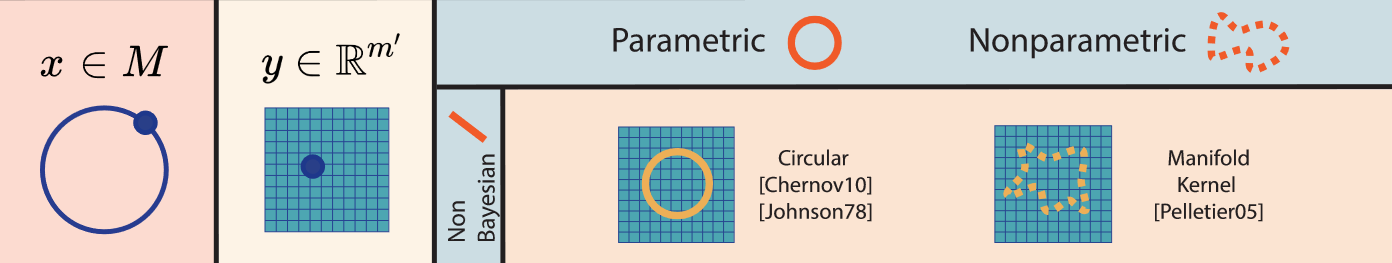
\includegraphics[width=0.8\textwidth]{images/regression_3.png}
  \end{figure}  
\end{frame}

\subsection{Non-Euclidean to non-Euclidean}
\begin{frame}{Classification of regression algorithms}{Non-Euclidean to non-Euclidean}
\begin{itemize}
  \item Project data to the tangent space of $M$, do PCA there to get some lower-dimensional representation in $\mathbb{R}^k$, then use Euclidean $\mathbb{R}^k \to M'$ algorithm
\end{itemize}
  \begin{figure}[h!]
    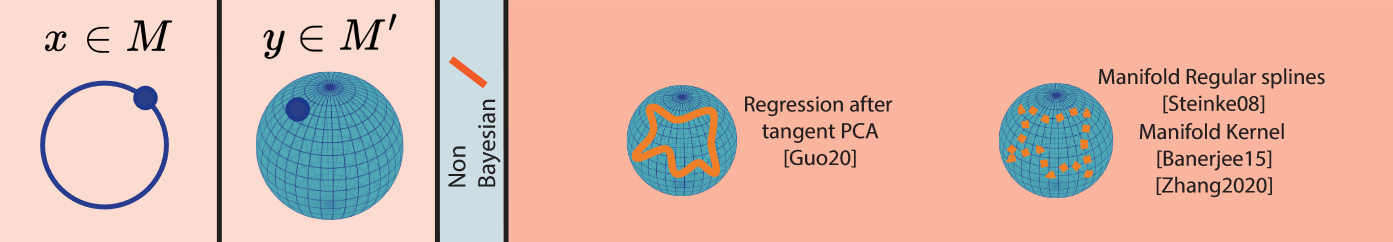
\includegraphics[width=0.8\textwidth]{images/regression_4.png}
  \end{figure}  
\end{frame}


\section{Survey of neural network layers}
\begin{frame}{Survey of neural network layers}{Geometric structure}
  \begin{itemize}
    \item Not that different from regression
    \item \textbf{ManifoldNet} (Chakraborty, et al., 2022): using weighted Fréchet mean as a convolution with manifold input/manifold output 
  \end{itemize}
  \begin{figure}[h!]
    \centering
    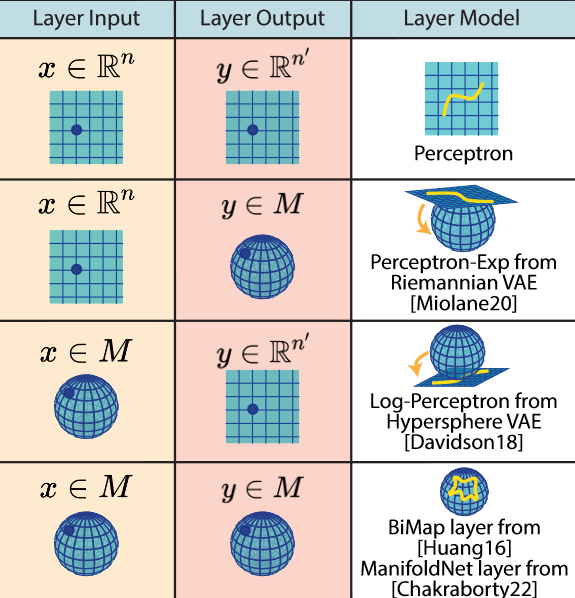
\includegraphics[width=0.4\textwidth]{images/nn_geometric.png}
  \end{figure}
\end{frame}

\begin{frame}{Survey of neural network layers}{Algebraic structure}
\begin{itemize}
  \item Given a group $G$ acting on input space $X$ with $\circ : G \times X \to X$ and output space $Y$ with $\cdot : G \times Y \to Y$, if $f(x, \theta) \in Y$ is the layer, then 
  \item \textbf{Invariance constraint} $f(g \circ x) = f(x)$, e.g. $X = \mathbb{R}^n$, $G = S_n$ permutation group, we can take all weights $\theta$ to be the same, then our NN is permutation invariant 
  \item \textbf{Equivariance constraint} $x$ is an image, $f(g \circ x) = g \cdot f(x)$, e.g. convolutional layer where $G$ is a group of translations 
\end{itemize}
\begin{figure}[h!]
  \centering
  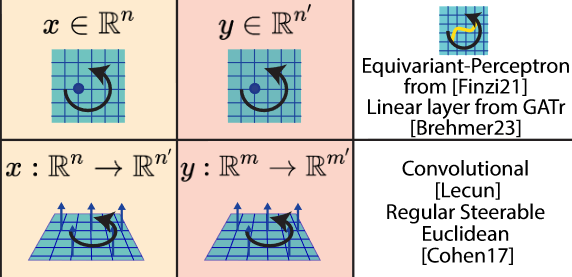
\includegraphics[width=0.5\textwidth]{images/nn_algebraic.png}
\end{figure}
\end{frame}

\begin{frame}{Survey of neural network layers}{Topological structure}
\begin{figure}[h!]
  \centering
  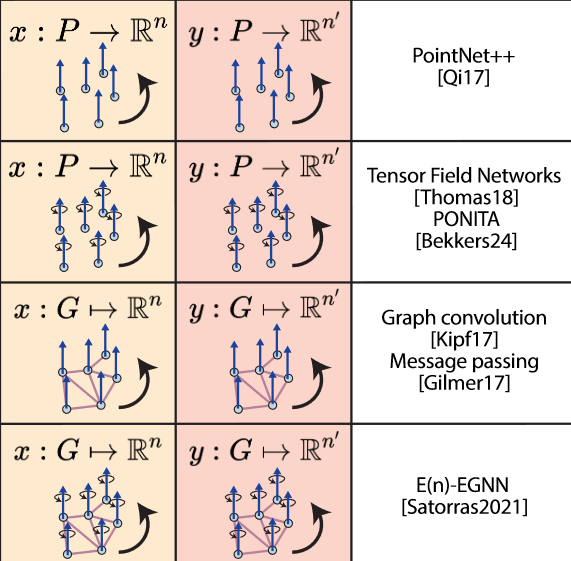
\includegraphics[width=0.5\textwidth]{images/nn_topological.png}
\end{figure}
\end{frame}
  

\section{Review}
\begin{frame}{Review}
\begin{figure}[h!]
  \centering
  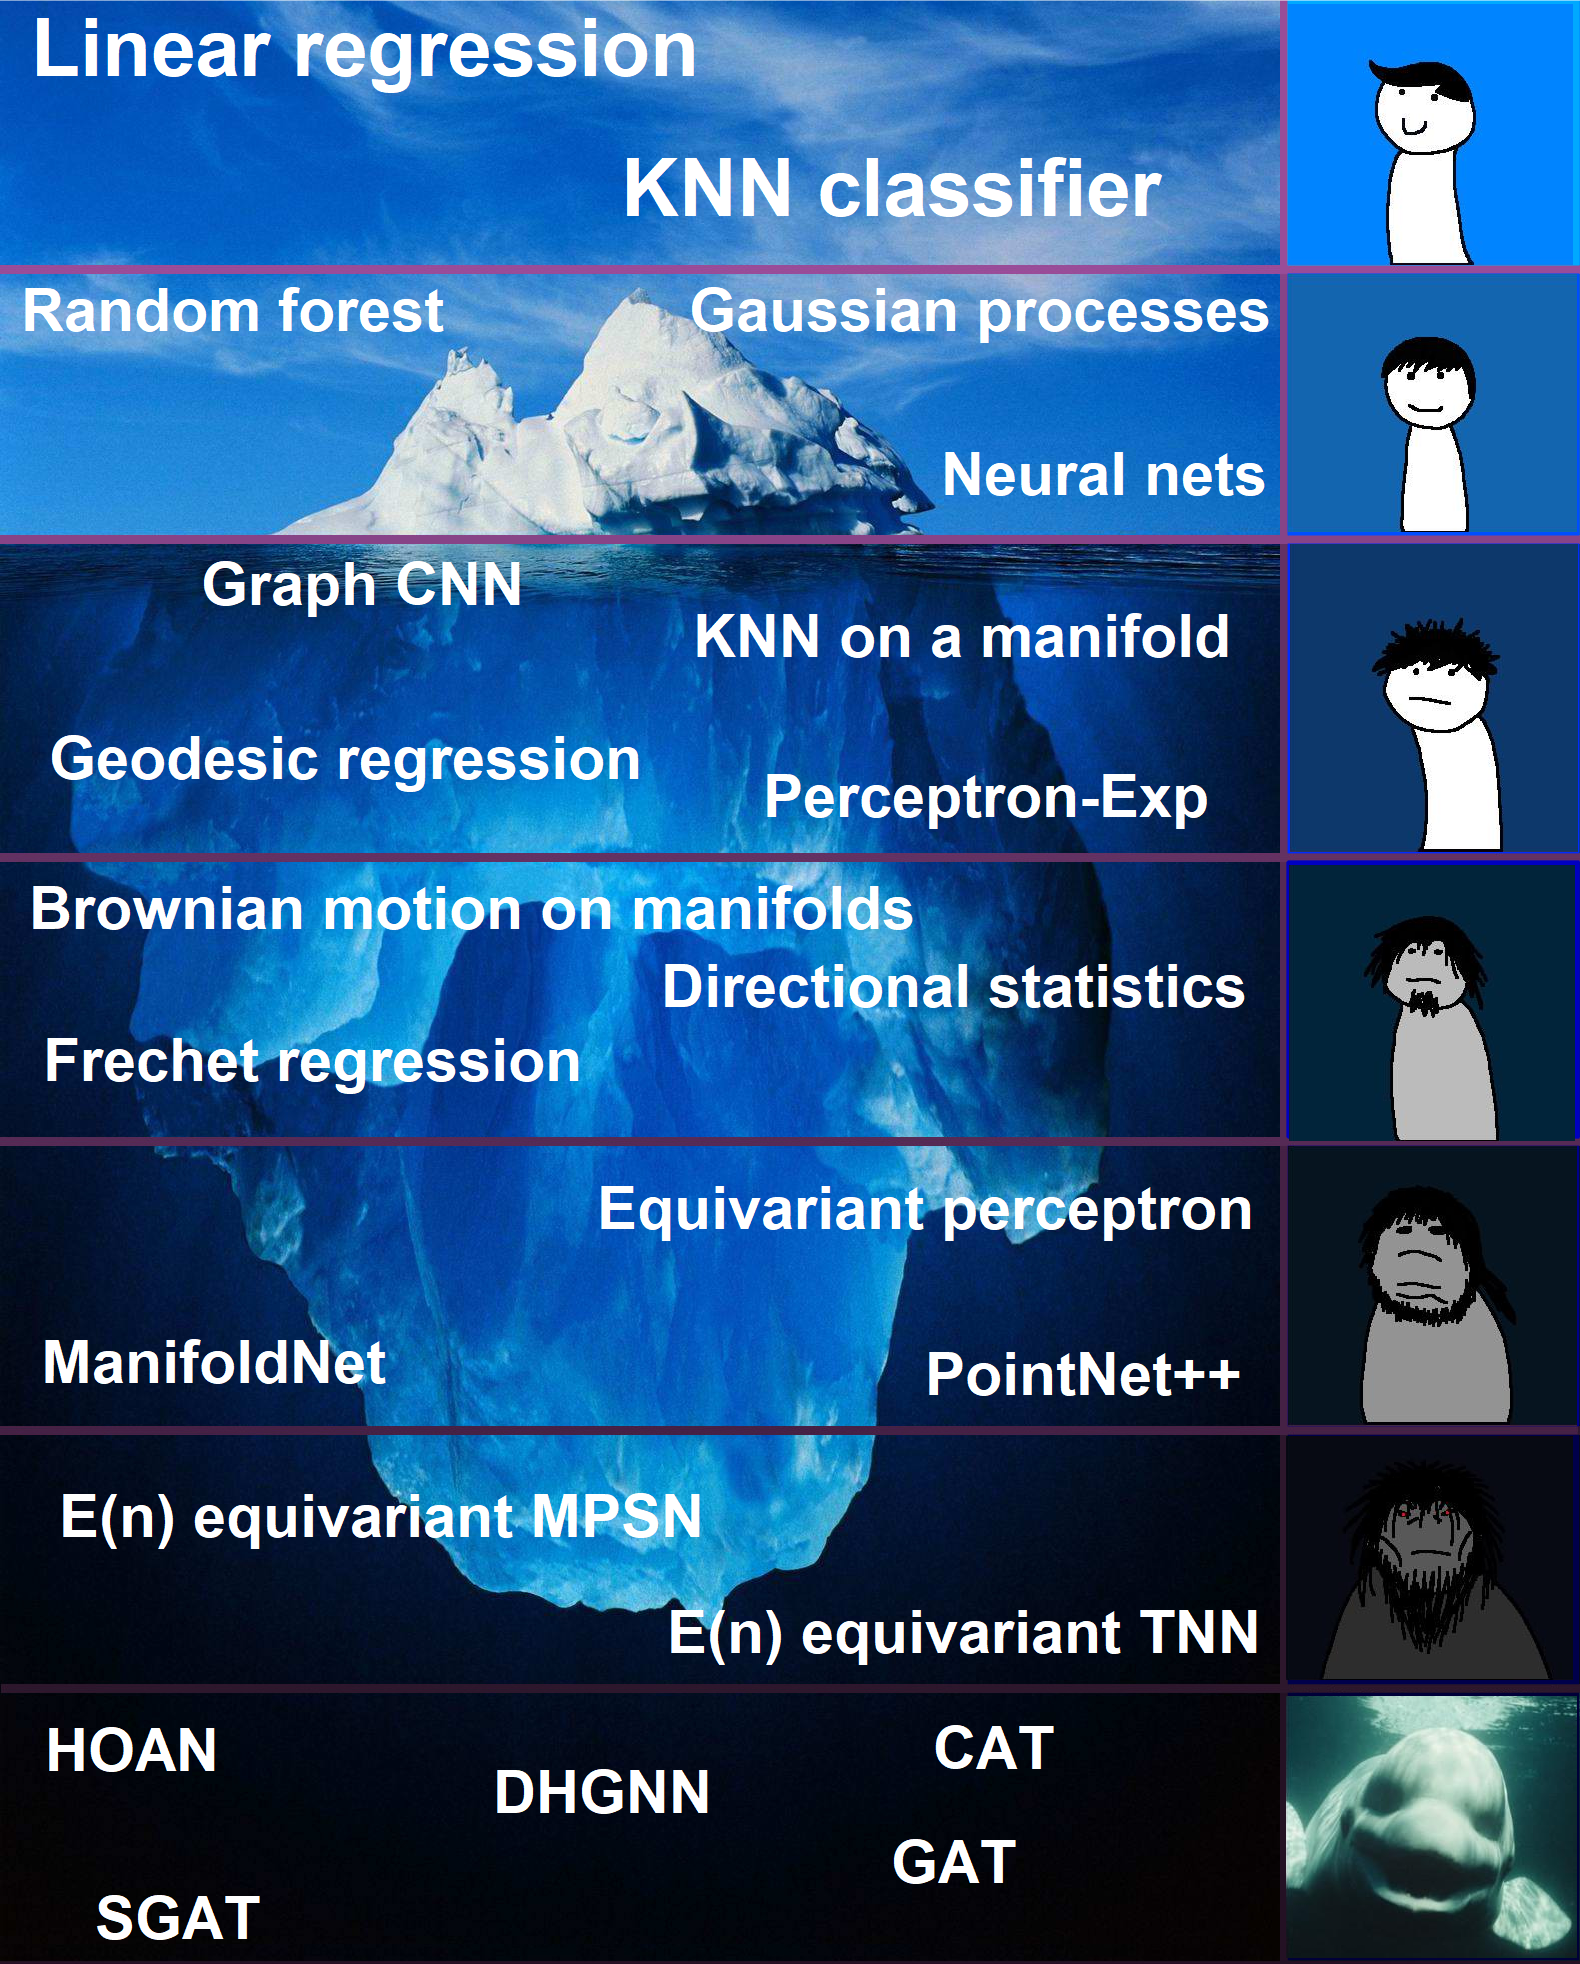
\includegraphics[width=0.5\textwidth]{images/7evxqcw8hoe51.png}
\end{figure}
\end{frame}

\begin{frame}{Software}
  \begin{enumerate}
    \item Geomstats https://geomstats.github.io/index.html -- statistics, and machine learning on nonlinear manifolds
    \item Manopt https://pymanopt.org/ -- optimization toolkit, also available for MATLAB and Julia
  \end{enumerate}
\end{frame}

\begin{frame}{Other references}
  \begin{enumerate}
    \item \textit{Geodesic Regression on Riemannian Manifolds}, Thomas Fletcher
    \item \textit{Fréchet Regression for Random Objects with
    Euclidean Predictors}, Alexander Petersen \& Hans-Georg Muller 
    \item \textit{A Practical Method for Constructing Equivariant Multilayer Perceptrons for Arbitrary Matrix Groups}, Finzi et al.
    \item \textit{Topics in circular statistics}, Jammalamadaka 
    \item \textit{Introduction to Smooth Manifolds}, John M. Lee
    \item \textit{An Introduction to
    Optimization on Smooth Manifolds}, Nicolas Boumal 
  \end{enumerate}
\end{frame}



\end{document}